%% main file
%%


\documentclass[ebook,10pt,oneside,openany,final, french]{memoir}

\usepackage{babel}
\usepackage[utf8]{inputenc}

\usepackage[final]
           {listings}     % code listings
\usepackage{relsize}      % provide relative font size changes
\usepackage{underscore}   % remove special status of '_' in ordinary text
\usepackage{verbatim}     % improved verbatim environment
\usepackage{parskip}      % handle non-indented paragraphs "properly"
\usepackage{array}        % new column definitions for tables
\usepackage[normalem]{ulem}
\usepackage{color}        % define colors for strikeouts and underlines
\usepackage{amsmath}      % additional math symbols
\usepackage{mathrsfs}     % mathscr font
\usepackage{microtype}
\usepackage{multicol}
\usepackage{xspace}
\usepackage{fixme}
\usepackage{lmodern}
\usepackage[T1]{fontenc}
\usepackage[pdftex,
            pdftitle={Deep networks for character recognition},
            pdfsubject={},
            pdfcreator={Vincent CHAMBRIN},
            bookmarks=true,
            bookmarksnumbered=true,
            pdfpagelabels=true,
            pdfpagemode=UseOutlines,
            pdfstartview=FitH,
            linktocpage=true,
            colorlinks=true,
            linkcolor=blue,
            plainpages=false
           ]{hyperref}
\usepackage{memhfixc}     % fix interactions between hyperref and memoir
\usepackage{xstring}
\usepackage{caption}
\usepackage{subcaption}
\usepackage{wrapfig}
\usepackage{amsfonts}
\usepackage{stmaryrd}
\usepackage{cite}
\usepackage{mathtools}


\usepackage{amsthm}
\newtheorem{theorem}{Théorème}[section]
\newtheorem{corollary}{Corollaire}[theorem]
\newtheorem{lemma}[theorem]{Lemme}
\newtheorem{proposition}[theorem]{Proposition}
\newtheorem{remark}{Remarque}
\newtheorem{definition}{Définition}



%%--------------------------------------------------
%%  set page size, type block size, type block position

\setstocksize{11in}{8.5in}
\settrimmedsize{11in}{8.5in}{*}
\setlrmarginsandblock{1in}{1in}{*}
\setulmarginsandblock{1in}{*}{1.618}

%%--------------------------------------------------
%%  set header and footer positions and sizes

\setheadfoot{\onelineskip}{2\onelineskip}
\setheaderspaces{*}{2\onelineskip}{*}

%%--------------------------------------------------
%%  make miscellaneous adjustments, then finish the layout
\setmarginnotes{7pt}{7pt}{0pt}
\checkandfixthelayout


%%--------------------------------------------------
%%  create chapter style

\makechapterstyle{chapterStyle}{%
  \renewcommand{\beforechapskip}{\onelineskip}
  \renewcommand{\afterchapskip}{\onelineskip}
  \renewcommand{\chapternamenum}{}
  \renewcommand{\chapnamefont}{\chaptitlefont}
  \renewcommand{\chapnumfont}{\chaptitlefont}
  \renewcommand{\printchapternum}{\chapnumfont\thechapter\quad}
  \renewcommand{\afterchapternum}{}
}

%%--------------------------------------------------
%%  create page styles

\makepagestyle{pageStyle}
\makeevenhead{pageStyle}{}{}{}
\makeoddhead{pageStyle}{}{}{}
\makeevenfoot{pageStyle}{\leftmark}{}{\thepage}
\makeoddfoot{pageStyle}{\leftmark}{}{\thepage}

\makeatletter
\makepsmarks{pageStyle}{%
  \let\@mkboth\markboth
  \def\chaptermark##1{\markboth{##1}{##1}}%
  \def\sectionmark##1{\markboth{%
    \ifnum \c@secnumdepth>\z@
      \textsection\space\thesection
    \fi
    }{\rightmark}}%
  \def\subsectionmark##1{\markboth{%
    \ifnum \c@secnumdepth>\z@
      \textsection\space\thesubsection
    \fi
    }{\rightmark}}%
  \def\subsubsectionmark##1{\markboth{%
    \ifnum \c@secnumdepth>\z@
      \textsection\space\thesubsubsection
    \fi
    }{\rightmark}}%
  \def\paragraphmark##1{\markboth{%
    \ifnum \c@secnumdepth>\z@
      \textsection\space\theparagraph
    \fi
    }{\rightmark}}}
\makeatother

\aliaspagestyle{chapter}{pageStyle}

%%--------------------------------------------------
%%  set heading styles for main matter
\newcommand{\beforeskip}{-.7\onelineskip plus -1ex}
\newcommand{\afterskip}{.3\onelineskip minus .2ex}

\setbeforesecskip{\beforeskip}
\setsecindent{0pt}
\setsecheadstyle{\large\bfseries\raggedright}
\setaftersecskip{\afterskip}

\setbeforesubsecskip{\beforeskip}
\setsubsecindent{0pt}
\setsubsecheadstyle{\large\bfseries\raggedright}
\setaftersubsecskip{\afterskip}

\setbeforesubsubsecskip{\beforeskip}
\setsubsubsecindent{0pt}
\setsubsubsecheadstyle{\normalsize\bfseries\raggedright}
\setaftersubsubsecskip{\afterskip}

\setbeforeparaskip{\beforeskip}
\setparaindent{0pt}
\setparaheadstyle{\normalsize\bfseries\raggedright}
\setafterparaskip{\afterskip}

\setbeforesubparaskip{\beforeskip}
\setsubparaindent{0pt}
\setsubparaheadstyle{\normalsize\bfseries\raggedright}
\setaftersubparaskip{\afterskip}


%%--------------------------------------------------
%%  set footnote style
\footmarkstyle{\smaller#1) }

%%--------------------------------------------------
% set style for main text
\setlength{\parindent}{0pt}
\setlength{\parskip}{1ex}
\setlength{\partopsep}{-1.5ex}

%%--------------------------------------------------
%%  set caption style and delimiter
\captionstyle{\centering}
\captiondelim{ --- }
% override longtable's caption delimiter to match
\makeatletter
\def\LT@makecaption#1#2#3{%
  \LT@mcol\LT@cols c{\hbox to\z@{\hss\parbox[t]\LTcapwidth{%
    \sbox\@tempboxa{#1{#2 --- }#3}%
    \ifdim\wd\@tempboxa>\hsize
      #1{#2 --- }#3%
    \else
      \hbox to\hsize{\hfil\box\@tempboxa\hfil}%
    \fi
    \endgraf\vskip\baselineskip}%
  \hss}}}
\makeatother

%%--------------------------------------------------
%% set global styles that get reset by \mainmatter
\newcommand{\setglobalstyles}{
  \counterwithout{footnote}{chapter}
  \counterwithout{table}{chapter}
  \counterwithout{figure}{chapter}
  \renewcommand{\chaptername}{}
  \renewcommand{\appendixname}{Annexe }
}

%%--------------------------------------------------
%% set section numbering limit, toc limit
\maxsecnumdepth{subparagraph}
\setcounter{tocdepth}{1}



\newcommand*{\transp}[2][-3mu]{\ensuremath{\mskip1mu\prescript{\smash{\mathrm t\mkern#1}}{}{\mathstrut#2}}}%
\newcommand{\vecnorm}[1]{\left\Vert #1\right\Vert}
\newcommand{\dotprod}[2]{\langle #1 | #2 \rangle }

\newcommand{\CodeStyle}{\ttfamily}
\newcommand{\CodeStylex}[1]{\texttt{#1}}

\newcommand{\tcode}[1]{\CodeStylex{#1}}

\newcommand{\Cpp}{\texorpdfstring{C\kern-0.05em\protect\raisebox{.35ex}{\textsmaller[2]{+\kern-0.05em+}}}{C++}\xspace}
\newcommand{\Python}{Python\xspace}

% Non French Words
\newcommand{\nfw}[1]{\emph{#1}\xspace}


\newcommand{\bigoh}[1]{\ensuremath{\mathscr{O}(#1)}}

%% Ranges
\newcommand{\Range}[4]{\tcode{#1#3,~\brk{}#4#2}\xspace}
\newcommand{\crange}[2]{\Range{[}{]}{#1}{#2}}
\newcommand{\brange}[2]{\Range{(}{]}{#1}{#2}}
\newcommand{\orange}[2]{\Range{(}{)}{#1}{#2}}
\newcommand{\range}[2]{\Range{[}{)}{#1}{#2}}



%%--------------------------------------------------
%% Environments for code listings.

% We use the 'listings' package, with some small customizations.  The
% most interesting customization: all TeX commands are available
% within comments.  Comments are set in italics, keywords and strings
% don't get special treatment.
\lstset{language=Python,
        basicstyle=\small\CodeStyle,
        xleftmargin=1em,
        showstringspaces=false,
        commentstyle=\itshape\rmfamily,
        columns=flexible,
        keepspaces=true,
        literate=
{á}{{\'a}}1
{à}{{\`a}}1
{ã}{{\~a}}1
{é}{{\'e}}1
{è}{{\`e}}1
{ê}{{\^e}}1
{í}{{\'i}}1
{ó}{{\'o}}1
{ô}{{\^o}}1
{õ}{{\~o}}1
{ú}{{\'u}}1
{ü}{{\"u}}1
{ç}{{\c{c}}}1}

% Our usual abbreviation for 'listings'.  Comments are in
% italics.  Arbitrary TeX commands can be used if they're
% surrounded by @ signs.
\newcommand{\CodeBlockSetup}{
 \lstset{escapechar=@}
 \renewcommand{\tcode}[1]{\textup{\CodeStylex{##1}}}
}

\lstnewenvironment{codeblock}{\CodeBlockSetup}{}


%%--------------------------------------------------
%% Indented text
\newenvironment{indented}
{\list{}{}\item\relax}
{\endlist}





\makeindex


%%--------------------------------------------------
%% fix interaction between hyperref and other
%% commands
\pdfstringdefDisableCommands{\def\smaller#1{#1}}
\pdfstringdefDisableCommands{\def\textbf#1{#1}}
\pdfstringdefDisableCommands{\def\raisebox#1{}}
\pdfstringdefDisableCommands{\def\hspace#1{}}


\begin{document}
\chapterstyle{chapterStyle}
\pagestyle{pageStyle}

\frontmatter


\thispagestyle{empty}
\begingroup
\def\hd{\begin{tabular}{ll}
          \textbf{Date:}             & \today       \\
          \textbf{Auteur:}           & Vincent CHAMBRIN      \\
                                     & Fabien ROUILLON      \\
          \end{tabular}
}
\newlength{\hdwidth}
\settowidth{\hdwidth}{\hd}
\hfill\begin{minipage}{\hdwidth}\hd\end{minipage}
\endgroup

\vspace{2.5cm}
\begin{center}
\textbf{\Huge Projet Mathématiques et Applications} \\ 
\vspace{1cm}
\Huge{\textit{Deep networks for character recognition}}
\end{center}

\vfill


\newpage



\chapter{Sommaire}

Le but de ce projet est d'étudier l'utilisation de réseaux de neurones 
profonds pour la reconnaissance de caractères manuscrits. 
Différentes méthodes de classifications seront utilisées et comparées à un réseau 
de neurones simple et à des algorithmes n'utilisant pas de réseaux de neurones.
Le langage \Python sera utilisé pour l'écriture des programmes, ce dernier 
fournissant bon nombre de bibliothèques de \nfw{machine learning}. \\
Pour mieux comprendre les algorithmes et idées mis en jeux, une brève 
introduction aux principes des réseaux de neurones sera présentée. 
%Une interface graphique permettant de mieux visualiser les résultats sera 
%également présentée.

\vspace{1cm}

Mots-clés: réseaux de neurones, \nfw{machine learning}, \nfw{deep networks}, reconnaissance de caractères, \Python.

\vfill


\newpage
\let\oldleftmark=\leftmark
\renewcommand{\leftmark}{Table des matières}

\setcounter{tocdepth}{4}
\tableofcontents

\pagebreak
\let\leftmark=\oldleftmark

\mainmatter
\setglobalstyles


\chapter{Introduction}

La reconnaissance de caractères, ou plus généralement de textes manuscrits, est 
un domaine en pleine expansion. 
De nombreux géants de l'informatique comme Google, Apple ou Microsoft se battent pour 
offrir à leurs utilisateurs (et probablement à d'autres fins) le meilleur système 
de reconnaissance de texte. Les utilisations sont nombreuses :
\begin{itemize}
  \item application de prises de notes;
  \item saisie de formulaires;
  \item saisie d'une adresse pour le système GPS de certaines voitures;
  \item reconnaissance d'adresse postale sur les enveloppes;
  \item reconnaissance d'un montant sur les chéques.
\end{itemize}

\vspace{1em}

Dans le cadre de ce projet, on se contentera de tenter de reconnaître des chiffres. 
On utilisera pour cela le jeu de données MNIST, qui est un jeu de données contenant 
60000 images d'apprentissage et 10000 images de test. Ces images, représentants des 
chiffres écrits à la main, sont en niveaux de gris et font 28 pixels par 28 pixels.
Elles sont issues de deux jeux de données collectés par le NIST 
(United States' National Institute of Standards and Technology). 
A chaque image est associé un label (i.e.\/ le chiffre représenté). 
Ce jeu de données est pratiquement devenu un standard dans le monde de la 
reconnaissance de caractères.

Ce rapport est découpé en plusieurs parties. Dans un premier temps, une introduction 
sur les réseaux de neurones permettra de se familiariser avec ces derniers. 
On sera alors en mesure d'écrire nous-même les algorithmes pour les réseaux les 
plus simples et nous pourrons construire un premier réseau permettant de répondre 
au problème de classification que l'on se pose. \\
Ensuite, nous pourrons mettre en oeuvre des techniques de`\nfw{machine learning} 
plus poussés et plus adaptés à notre domaine. On commencera pour cela par 
étudier certaines techniques propres au problème de reconnaissance de caractères
(l'extraction de \nfw{features}).
Enfin, nous nous pencherons sur l'utilisation de réseaux de neurones convolutionnels, 
ces derniers étant particulièrement adaptés aux problèmes de vision par ordinateur 
et de traitement d'image.


\chapter{Les réseaux de neurones}

Dans cette partie, nous présentons de manière simplifiée les réseaux de neurones 
et comment les utiliser pour résoudre notre problème de classification.
Ce chapitre s'inspire fortement de \textit{Neural Networks and Deep Learning}\cite{neuralnetworksanddeeplearning} 
et en reprend les notations.


\section{Le modèle du perceptron}



\begin{definition}[Fonction de Heaviside]
On appelle fonction de Heaviside la fonction $H$ définie de $\mathbb{R}$ dans $\{0, 1\}$ par :
\[
H(x) = 
\begin{cases}
 1, \text{ si } x \geq 0 \\
 0, \text{ sinon.} 
 \end{cases}
\]
\end{definition}

\begin{figure}[h]
  \centering
  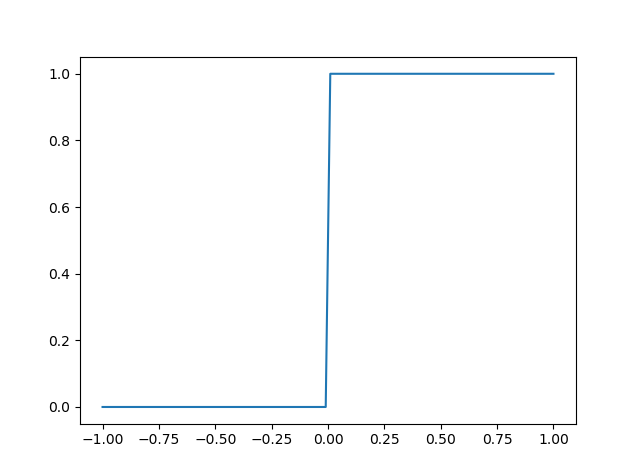
\includegraphics[scale=0.5]{assets/heaviside}
  \caption{La fonction échelon unité, ou fonction de Heaviside.}
  \label{fig:heaviside}
\end{figure}

Le but du perceptron est de modéliser le comportement du neurone biologique. 
Ce dernier est stimulé par des signaux qui lui parviennent par ses dendrites et, si 
la stimulation est suffisament importante, renvoie un signal à d'autres neurones au travers de son axone.

En notant $x_1, x_2, \dots, x_n$ ces stimulations, qui sont donc les entrées du perceptron, et 
$w_1, w_2, \dots, w_n$ les pondérations associées à ces entrées, on peut simplement exprimer le 
comportement du perceptron par :

\[
\text{sortie } =
\begin{cases}
 1 \text{ si } w \cdot x  \geq \text{ seuil} \\
 0 \text{ si } w \cdot x  < \text{ seuil.} 
 \end{cases}
\]

Par la suite, on préférera, plutôt que de considérer un seuil, considérer 
une quantité $b$ que l'on appelera \textit{biais} définie par $b = -\text{seuil}$, et on écrira:

\[
\text{sortie } = H(w \cdot x + b)
\]

Les perceptrons peuvent être utilisés pour coder des fonctions logiques. 
Par exemple, en prenant $w = (1, 1)$ et $b = -2$, notre perceptron code 
un ET logique (avec la convention 0 pour FAUX et 1 pour VRAI).

\begin{figure}[h]
  \centering
  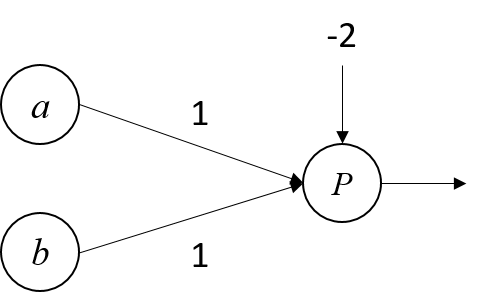
\includegraphics[scale=0.5]{assets/and-perceptron}
  \caption{Fonction ET logique.}
  \label{fig:and-perceptron}
\end{figure}

De même, en prenant $w = (-2, -2)$ et $b = 3$, on code la fonction NAND 
(négation du ET logique). Pour s'en convaincre, on peut dresser le tableau 
des sorties en fonction de toutes les entrées possibles comme cela est fait 
dans la table \ref{table:nand-perceptron}.

\begin{table}[h]
  \centering
\begin{tabular}{|c|c|c|c|}
\hline
$x_1$ & $x_2$ & $wx + b$ & Sortie \\
\hline
0     & 0     & 3        & 1 \\  
0     & 1     & 1        & 1 \\  
1     & 0     & 1        & 1 \\  
0     & 0     & -1       & 0 \\   
\hline
\end{tabular} 
  \caption{Table de vérité du perceptron.}
  \label{table:nand-perceptron}
\end{table}

\begin{figure}[h]
  \centering
  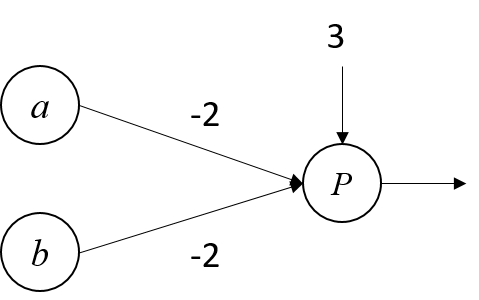
\includegraphics[scale=0.5]{assets/nand-perceptron}
  \caption{Fonction NAND.}
  \label{fig:nand-perceptron}
\end{figure}

Comme la fonction NAND permet de coder n'importe quelle fonction logique, 
on en déduit qu'en utilisant la sortie de perceptrons comme entrées d'autres 
perceptrons, on peut construire n'importe quelle fonction logique.

Cette idée d'empiler des couches de perceptrons pour coder une fonction logique 
conduit naturellement à l'idée que l'on pourrait se faire d'un réseau de neurones.

\begin{figure}[h]
  \centering
  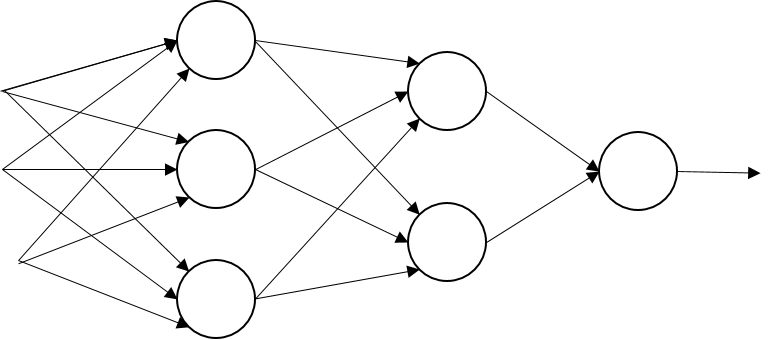
\includegraphics[scale=0.5]{assets/perceptron-network}
  \caption{Un réseau de perceptrons.}
  \label{fig:perceptron-network}
\end{figure}

Jusqu'à présent, nous nous sommes restreint à des entrées binaires (0 ou 1) 
codant des valeurs logiques. Ceci n'est pas nécessaire : les entrées d'un perceptron 
peuvent très bien être des réels.
Plaçons nous, pour les exemples qui vont suivres, dans $\mathbb{R}^2$. 
Pour chaque point $(x, y)$ du plan, on donnera $x$ comme première entrée d'un 
perceptron et $y$ comme seconde entrée. 
Le perceptron ayant pour paramètres $w=(\alpha_x, \alpha_y)$ et $b$ va alors 
séparer l'espace en deux plans par la droite d'équation $\alpha_y y + \alpha_x x + b = 0$. 
Les points tels que $\alpha_y y + \alpha_x x + b \geq 0$ auront pour sortie $1$, et 
les autres auront pour sortie $0$.

Ceci est illustré par la figure \ref{fig:perceptron-example1} dans laquelle la 
partie verte correspond à une sortie positive du perceptron dès lors que $y \geq x$.

\begin{figure}[h]
  \centering
  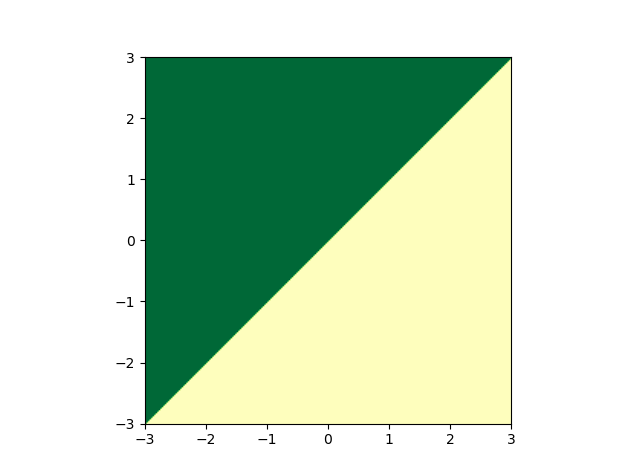
\includegraphics[scale=0.5]{assets/perceptron-example1}
  \caption{Découpage du plan en deux par un perceptron.}
  \label{fig:perceptron-example1}
\end{figure}


En utilisant plusieurs perceptron, on va pouvoir effectuer plusieurs sous-découpage 
de l'espace, et en utilisant un ET logique dans une dernière couche 
on va pouvoir récuperer la partie de l'espace 
correspondant à l'intersection de toutes les parties correspondants aux sorties 
positives des perceptrons de la couche précédente.

\begin{figure}[h]
  \centering
  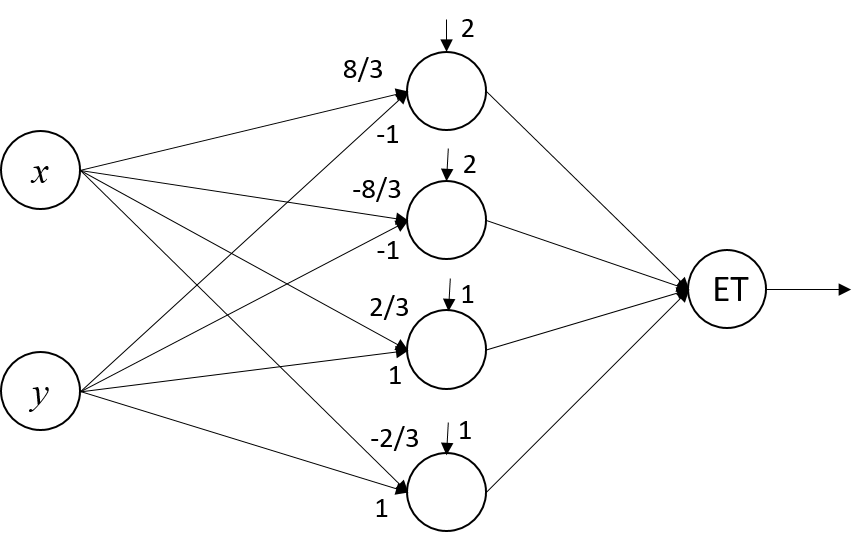
\includegraphics[scale=0.5]{assets/perceptron-network-example2}
  \caption{Un premier réseau de perceptrons.}
  \label{fig:perceptron-network-example2}
\end{figure}

\begin{figure}[h]
  \centering
  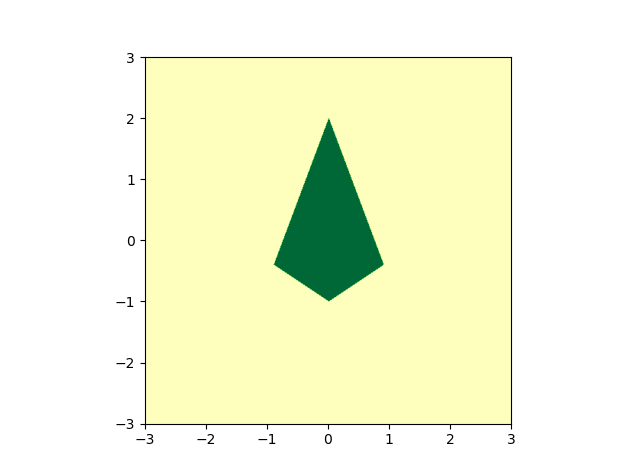
\includegraphics[scale=0.5]{assets/perceptron-example2}
  \caption{Découpage du plan par un réseau de perceptrons.}
  \label{fig:perceptron-example2}
\end{figure}

Cette approche a ses limites car elle ne permet d'obtenir qu'une partie convexe 
du plan. Pour obtenir des parties plus complexes (e.g.\/ non convexes, ou non 
fortement connexes), on peut utiliser d'autres fonctions logiques, comme le OU. 

\begin{figure}[h]
  \centering
  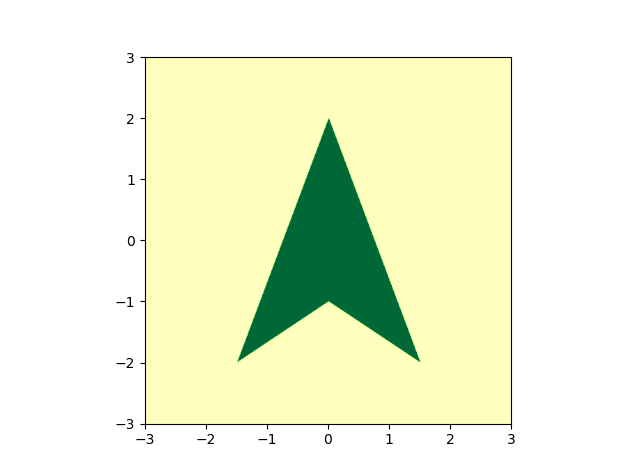
\includegraphics[scale=0.5]{assets/perceptron-example3}
  \caption{Un découpage non convexe du plan avec un réseau de perceptrons à deux couches.}
  \label{fig:perceptron-example3}
\end{figure}

Il n'est pas difficile d'imaginer que l'on puisse étendre ce que l'on vient de faire en 
2 dimensions à un nombre plus grand de dimensions; et avec non plus une seule sortie 
mais plusieurs (correspondant par exemple chacune à une classe, à un chiffre que l'on 
souhaite reonnaître).
On pourrait donc en théorie construire un réseau de neurones avec des perceptrons 
qui serait capable de reconnaître des chiffres. 
L'un des problèmes de cette approche est qu'il faudrait déjà connaître les coefficients 
(ou paramètres) de l'ensemble des perceptrons du réseau.
On pourrait alors avoir envie d'écrire un algorithme permettant de construire un tel 
réseau. On peut imaginer plusieurs principes pour cet algorithme :`
\begin{enumerate}
  \item tester tous les coefficients possibles pour les perceptrons;
  \item partir d'une configuration aléatoire et modifier petit à petit les coefficients 
        jusqu'à obtenir un résultat satisfaisant.
\end{enumerate}

La première idée est tout simplement irréalisable car il y a une infinité de valeurs 
possibles pour chaque coefficient du réseau. On pourrait penser à prendre une 
approche probabiliste en testant un certain nombre de réseaux et en espérant tomber sur 
un bon; ce qui paraît néanmoins très improbable ! 
La deuxième idée n'est également pas envisageable car elle souffre d'un problème difficile 
à gérer. La discontinuité de la fonction de Heaviside fait qu'un petit changement de coefficient 
peut faire passer la sortie d'un neurone de 0 à 1 ce qui peut correspondre à un changement 
significatif de l'entrée des neurones de la couche suivante. Il est donc compliqué d'évaluer 
l'impact d'un changement à une couche donnée sur les couches qui suivent.

L'idée qui va être explorée dans les paragraphes suivants est d'utiliser une autre fonction, 
appelée fonction d'activation, que la fonction échelon d'Heaviside; et de faire en sorte que 
cette fonction d'activation soit dérivable (et donc continue) pour pouvoir utiliser des 
résultats d'analyse et pouvoir ainsi estimer l'impact du changement d'un coefficient.
On sera alors en mesure de modifier un réseau généré aléatoirement pour le faire résoudre 
notre problème de classification (on parlera d'apprentissage).



\section{Structure des réseaux de neurones}



\begin{definition}[Fonction sigmoïde]
On appelle fonction sigmoïde la fonction définie de $\mathbb{R}$ dans $[0, 1]$ par :
\[
\sigma(x) = \frac{1}{1 + e^{-x}}
\]
\end{definition}

On notera que $\lim_{x \to +\infty} \sigma(x) = 1$ et $\lim_{x \to -\infty} \sigma(x) = 0$. 
Ainsi, asymptotiquement, la fonction sigmoïde a le même comportement que la fonction 
de Heaviside.

Entre les deux, on a un comportement qui diffère fortement du perceptron avec notamment 
la non discontinuité en 0 et $\sigma(0) = \frac{1}{2}$. 
Dans le cadre de notre utilisation pour la classification on aura tendance 
à considérer que la sortie du neurone est à \textsc{vrai} dès qu'elle sera supérieure 
à une certaine valeur (typiquement $\frac{1}{2}$).

On a également quelques propriétés intéressantes de symétrie. En effet,

\[
\sigma'(x) = \frac{e^{-x}}{1 + e^{-x}} = \sigma(x) (1 - \sigma(x))
\]

\[
\sigma'(x) - \sigma'(-x) = \frac{e^{-x}(e^{2x} + 2 e^{x} + 1) - e^{x}(e^{-2x} + 2 e^{-x} + 1)}{(1+e^{-x})^2 (1+e^{x})^2} = 0
\]

ce qui signifie que la sigmoïde admet pour centre de symétrie le point $(0, \frac{1}{2})$.

Cette fonction a de plus l'avantage d'être dérivable en tout point (et de dérivée non nulle), 
ce qui nous servira plus tard dans le cadre de l'apprentissage.


\begin{definition}[Modélisation d'un neurone]
En notant $b$ le biais du neurone, $w$ son vecteur des poids et $\sigma$ sa fonction 
d'activation, on peut écrire la sortie $a$ d'un neurone en fonction de son entrée $x$ 
de la manière suivante:
\[
a = \sigma(w \cdot x + b)
\]
\end{definition}


\begin{definition}[Vectorisation d'une fonction]
Soit $f$ une fonction de $\mathbb{R} \mapsto \mathbb{R}$. 
On pose pour tout vecteur $x$ de $\mathbb{R}^n$ :
\[
f(x) = 
\begin{pmatrix}
f(x_1) \\
f(x_2) \\
\vdots \\
f(x_n)
\end{pmatrix}
\]
On dit que l'on vectorise la fonction $f$.
\end{definition}

\textbf{Achtung !} Par abus de notation, on utilise encore le nom de $f$ pour désigner 
cette fonction, mais il s'agit bien d'une fonction différente puisqu'elle est à valeurs 
de $\mathbb{R}^n$ dans $\mathbb{R}^n$. Cet abus nous est néanmoins utile pour définir 
simplement les couches d'un réseau de neurones.

On considère dans les définitions suivantes une couche d'un réseau de neurones 
constituée de $n$ neurones. On note $w_i$ le vecteur des poids associé à chaque neurone.
On a alors la définition suivante:
 
\begin{definition}[Matrice des poids]
En notant $w_i$ les vecteurs des poids de $n$ neurones, on définit par blocs 
la matrice $w$ des poids:
\[
w = 
\begin{pmatrix}
{w_1}^T \\
{w_2}^T \\
\vdots \\
{w_n}^T
\end{pmatrix}
\]
\end{definition}

On définit de manière analogue un vecteur des biais.

\begin{definition}[Vecteur des biais]
En notant $b_i$ les biais de $n$ neurones, on définit le vecteur des biais 
d'une couche d'un réseau de neurones par:
\[
b = 
\begin{pmatrix}
{b_1} \\
{b_2} \\
\vdots \\
{b_n}
\end{pmatrix}
\]
\end{definition}

On a alors la proposition suivante:

\begin{proposition}[Ecriture matricielle d'une couche]
Soit une couche d'un réseau constituée de $n$ neurones et ayant pour matrice 
des poids $w$ et pour vecteur des biais $b$. Si les neurones ont tous la même 
fonction d'activation $\sigma$, on peut écrire les sorties des neurones sous la 
forme d'un vecteur $a$ vérifiant:
\[
a = \sigma(w \cdot x + b)
\]
où les $a_i$ correspondent à la sortie du neurone $i$.
\end{proposition}

On notera que dans cette proposition, on utilise la version vectorisée de $\sigma$.
Une écriture équivalente est:
\[
\begin{pmatrix}
  a_1 \\
  a_2 \\
  \vdots \\
  a_n
\end{pmatrix}
 = 
\begin{pmatrix}
  \sigma(w_1 \cdot x + b_1) \\
  \sigma(w_2 \cdot x + b_2) \\
  \vdots \\
  \sigma(w_n \cdot x + b_n)
\end{pmatrix}
\]

En fait, cette écriture est identique à celle d'un unique neurone !
Elle est également intéressante d'un point de vue computationnelle : au lieu 
de calculer une à une les sorties des neurones, il est plus efficace de faire 
un calcul matriciel (les bibliothèques étant en général optimisées pour cela).
Cela permet également d'avoir un code plus simple (avec notamment moins de boucles).

Cette écriture permet également d'écrire de manière très condensée un réseau 
de neurones à plusieurs couches. 
En notant $w^{1}, w^{2}, \cdots, w^{L}$ les matrices de poids de $L$ couches de 
neurones, et $b^{1}, b^{2}, \cdots, b^{L}$ les vecteurs des biais associés, et 
en supposant que tous les neurones ont pour fonction d'activation $\sigma$, on a
\begin{equation}
\label{eq:condensed-multilayer-expression}
a = \sigma(b^{L} + w^{L} \cdot \sigma(b^{L-1} + w^{L-1} \cdot \sigma(\cdots)))
\end{equation}

Pour avoir une écriture plus lisible, on introduit la notion suivante qui 
permet de parler de la sortie pour toute couche:
\begin{definition}[Activation d'un neurone]
On appellera activation du neurone $j$ de la couche $l$ la quantité $a_{j}^{l}$ 
définie par:
\[
a_{j}^{l} = \sigma \left( \sum_{k} w_{jk}^{l} a_{k}^{l-1} + b_{j}^{l} \right)
\]
Il s'agit simplement de la sortie de ce neurone.
\end{definition}

On peut alors réécrire l'équation \ref{eq:condensed-multilayer-expression} de la 
manière suivante, la sortie du réseau étant le vecteur $a^{L}$.
\[
\begin{cases}
 a^{l} = \sigma(w^{l} \cdot a^{l-1} + b^{l}) \\
 a^{0} = x \\
\end{cases}
\]

On constate donc que l'on peut très facilement calculer la sortie d'un réseau 
de neurones par un algorithme itératif. 

Autre remarque importante: il n'est pas nécessaire que les $(w^{l})_{l \in \llbracket 1, L \rrbracket}$ 
aient les mêmes dimensions. Autrement dit, il peut y avoir un nombre différent 
de neurones dans chaque couche; le seule impératif est que les dimensions 
d'une couche à la suivante soient cohérentes.

En reprenant les notations précédentes, on a que $w_{jk}^{l}$ est le poids de la 
connexion reliant le $k$\textsuperscript{ème} neurone de la couche $(l-1)$ au 
$j$\textsuperscript{ème} neurone de la couche $l$.
De la même manière, $b_{j}^{l}$ est le biais du $j$\textsuperscript{ème} neurone 
de la couche $l$.



\section{Apprentissage par la descente de gradient}


On considère dans cette partie un réseau de neurones à $L$ couches, et on note 
encore $w^{1}, w^{2}, \cdots, w^{L}$ les matrices des poids et $b^{1}, \cdots, b^{L}$
les vecteurs des biais. 
On cherche dans cette partie à améliorer de manière itérative la valeur des 
coefficients du réseau pour améliorer les prédictions. 
On introduit pour cela une fonction de coût, croissante de l'erreur, et 
on se ramène à un problème d'optimisation.

\begin{definition}[Fonction de coût quadratique]
Soit $X$ un ensemble d'apprentissage de cardinal $n$. 
On note $a^{L}(x)$ la sortie du réseau de neurones pour l'entrée $x \in X$ et 
$y_{x}$ la sortie désirée. On définit la fonction de coût par:
\[
C(w, b) = \frac{1}{2n} \sum_{x} \vecnorm{y_{x} - a^{L}(x)}^2
\]
\end{definition}

On parle aussi de \textsc{MSE} pour \nfw{mean square error}.

Par la suite, et pour alléger les notations, on écrira souvent $a^{L}$ et $y$ 
au lieu de $a^{L}(x)$ et $y_x$.

Cette fonction à le bon goût d'être convexe. Ainsi, on peut la minimiser en annulant 
sa dérivée. 
Cependant cette fonction dépend de tous les $w^{l}$ et $b^{l}$ ainsi que de la fonction 
$\sigma$, le calcul de la dérivée et de son point d'annulation n'est donc pas facile.
C'est pourquoi on va opter pour un algorithme itératif qui, partant d'un point quelconque 
(i.e.\/ un couple $(w,b)$ donné), va progressivement s'approcher de la solution. 

L'un des algorithmes les plus simples est celui de la descente de gradient.
Partant d'un point $v = (w,b)$, on souhaite trouver $\Delta v$ telle que 
$C(v + \Delta v) \leq C(v)$. Cet algorithme propose de prendre 
$\Delta v = -\eta\nabla C(v)$ avec $\eta$ suffisament petit pour que 
l'on puisse s'assurer de diminuer le coût $C$ et suffisament grand pour que les 
effets soient significatifs.

L'algorithme peut donc se résumer sous la forme suivante:
\begin{enumerate}
  \item étant donné $v = (w, b)$, calculer $\nabla C(v)$;
  \item calculer $v' = v - \eta \nabla C(v)$;
  \item recommencer l'étape 1 avec $v'$.
\end{enumerate}
On itère jusqu'à ce que le coût soit proche de son minimum.

En pratique on utilisera une variante stochastique de l'algorithme. 
En effet, 
\[
C = \frac{1}{n} \sum_{x} C_x \qquad \text{avec} \quad C_x = \frac{1}{2} \vecnorm{y - a^{L}}^2
\]
sera d'autant plus long à calculer que $n$ (la taille de l'échantillon d'apprentissage) 
est grand.
C'est pourquoi on tirera $m < n$ entrées au hasard et on se contentera de calculer 
le coût et son gradient sur ce sous-échantillon.



\section{L'algorithme de rétro-propagation}


L'algorithme de descente de gradient évoqué précédemment est en principe 
très simple. Cependant, le calcul de $\nabla C(v)$ est loin d'être simple. 
Cette quantité dépend en effet de tous les $w_{jk}^{l}$ et les $b_{j}^{l}$.
On présente dans cette partie une manière simple de calculer cette quantité 
via l'algorithme de rétro-propagation. 
Il est cependant nécessaire d'introduire d'abord quelques quantités utiles.


\begin{definition}[Entrées pondérées d'un neurone]
On notera $z_{j}^{l}$ les entrées pondérées du neurone $j$ de la couche $l$.
\[
z_{j}^{l} = \sum_{k} w_{jk}^{l} a_{k}^{l-1} + b_{j}^{l}
\]
\end{definition}

De manière évidente, on a $a_{j}^{l} = \sigma(z_{j}^{l})$.


Comme on l'a vu dans la partie précédente, le coût $C$ s'écrit comme somme 
de coûts unitaires:
\[
C = \frac{1}{n} \sum_{x} C_x
\]
Dans cette partie, on s'intéressa seulement au calcul de la quantité $C_x$ pour un $x$ donné. 
La vrai coût $C$ et $\nabla C$ se calculant simplement en faisant la somme.
On se fixe donc un $x$ et, pour simplifier les notations, on notera $y = y_x$ 
la sortie voulu et $C = C_x$.

L'idée de l'algorithme de rétro-propagation est de partir d'une quantité que 
l'on peut facilement calculer à partir de la sortie du réseau (que l'on obtient 
en faisant un \nfw{feedforward}, c'est à dire en parcourant le réseau depuis la 
première couche jusqu'à la dernière) et de revenir en arrière (\nfw{backpropagation}) 
pour attribuer à chaque coefficient du réseau une part de l'erreur.

Notons $a^L$ la sortie du réseau, on a:
\[
C = \frac{1}{2} \vecnorm{y - a^L}^2 = \frac{1}{2} \sum_{j} (y_j - a_{j}^{L})^2
\]
On obtient donc très facilement le résultat suivant.
\[
\frac{\partial C}{\partial a_{j}^{L}} = (a_{j}^{L} - y_j)
\]
Que l'on écrira sous forme vectorielle.
\[
\nabla_a C = a^{L} - y 
\]

La principe de l'algorithme de rétro-propagation va être de partir de cette 
quantité et de parcourir les couches du réseau à l'envers pour calculer les 
dérivées partielles $\frac{\partial C}{\partial w_{jk}^{l}}$ et $\frac{\partial C}{\partial b_{j}^{l}}$.

\begin{definition}[Erreur d'un neurone]
On définit l'erreur au neurone $j$ de la couche $l$ par:
\[
\delta_{j}^{l} = \frac{\partial C}{\partial z_{j}^{l}}
\]
\end{definition}

Cette définition est posée de manière un peu arbitraire et permet simplement 
de simplifier l'écriture des calculs que nous ferrons plus tard. 
Une autre définition possible aurait été de prendre l'erreur comme étant égale 
à $\frac{\partial C}{\partial a_{j}^{l}}$. Cela ne change pas grand chose car on 
a la relation suivante (règle de la chaîne).

\[
\frac{\partial C}{\partial z_{j}^{l}} = \sum_{i} \frac{\partial C}{\partial a_{i}^{l}} \frac{\partial a_{i}^{l}}{\partial z_{j}^{l}}
= \sum_{i} \frac{\partial C}{\partial a_{i}^{l}} \frac{\partial \sigma(z_{i}^{l})}{\partial z_{j}^{l}} = \frac{\partial C}{\partial a_{j}^{l}} \sigma'(z_{j}^{l})
\]


\begin{definition}[Produit de Hadamard]
Soit $S$ et $T$ deux matrices (ou vecteurs) de même dimension, on appelle 
produit de Hadamard de $S$ et $T$, noté $S \odot T$ la matrice de même dimension 
que $T$ et donc les composantes sont les produits éléments par éléments des 
coefficients de $S$ et $T$, i.e.\/
\[
(S \odot T)_{ij} = S_{ij} \times T_{ij}
\]
\end{definition}



\begin{proposition}[Equations de la rétro-propagation]
On a les relations suivantes: \\
Erreur au niveau de la dernière couche: 
\begin{equation}
  \label{eq:bp1}
\delta^{L} = \nabla_{a} C \odot \sigma'(z^{L})
\end{equation}
Erreur au niveau de la couche $l$:
\begin{equation}
  \label{eq:bp2}
\delta^{l} = ((w^{l+1})^T \delta^{l+1}) \odot \sigma'(z^{l})
\end{equation}
Dérivées partielles par rapport aux biais:
\begin{equation}
  \label{eq:bp3}
\frac{\partial C}{\partial b_{j}^{l}} = \delta_{j}^{l}
\end{equation}
Dérivées partielles par rapport aux poids:
\begin{equation}
  \label{eq:bp4}
\frac{\partial C}{\partial w_{jk}^{l}} = a_{k}^{l-1} \delta_{j}^{l}
\end{equation}
\end{proposition}

Ces équations nous donnent une méthode simple pour calculer les dérivées partielles 
par rapport aux coefficients du réseau et permettent ainsi d'appliquer la méthode 
de la descente de gradient.

\begin{proof}[Preuve de l'équation \ref{eq:bp1}]
Il suffit de reprendre ce que l'on a fait précédemment (règle de la chaîne). 
\[
\delta_{j}^{L} = \frac{\partial C}{\partial z_{j}^{L}} =
 \sum_{i} \frac{\partial C}{\partial a_{i}^{L}} \frac{\partial a_{i}^{L}}{z_{j}^{L}} =
 \sum_{i} \frac{\partial C}{\partial a_{i}^{L}} \frac{\partial \sigma(z_{i}^{L})}{z_{j}^{L}} =
 \frac{\partial C}{\partial a_{j}^{L}} \sigma'(z_{j}^{L})
\]
Soit sous forme vectorielle,
\[
\delta^{L} = \frac{\partial C}{\partial a^{L}} \odot \sigma'(z^{L})
\]
quantité que l'on écrit $\nabla_{a} C \odot \sigma'(z^{L})$.
\end{proof}

\vspace{1em}

Le résultat \ref{eq:bp2} est certainement le plus intéressant car c'est lui qui permet 
de remonter le réseau pour attribuer les erreurs aux différentes couches. 
Il dit grossièrement que pour retrouver l'erreur à la couche $l$, il suffit 
d'appliquer la transposée de la matrice de poids de la couche $l+1$ à l'erreur 
sur cette même couche et de multiplier par la dérivée de la sigmoïde.

\begin{proof}[Preuve de l'équation \ref{eq:bp2}]
On applique un raisonnement similaire à la preuve précédente.
\begin{align}
  \delta_{j}^{l} &= \frac{\partial C}{\partial z_{j}^{l}} \\
                 &= \sum_{k} \frac{\partial C}{\partial z_{k}^{l+1}} \frac{\partial z_{k}^{l+1}}{\partial z_{j}^{l}} \\
				 &= \sum_{k} \frac{\partial z_{k}^{l+1}}{\partial z_{j}^{l}} \delta_{k}^{l+1}
\end{align}
On se remémore ensuite l'expression de $z_{k}^{l+1}$:
\[
z_{k}^{l+1} = \sum_{i} w_{ki}^{l+1} a_{i}^{l} + b_{k}^{l+1} = \sum_{i} w_{ki}^{l+1} \sigma(z_{i}^{l}) + b_{k}^{l+1}
\]
Ce qui nous permet d'obtenir
\[
\frac{\partial z_{k}^{l+1}}{\partial z_{j}^{l}} = w_{kj}^{l+1} \sigma'(z_{j}^{l})
\]
On obtient donc le résultat voulu
\[
\delta_{j}^{l} = \sum_{k} w_{kj}^{l+1} \delta_{k}^{l+1} \sigma'(z_{j}^{l})
\]
\end{proof}

\vspace{1em}

Les deux derniers résultats servent à relier les quantités calculées aux 
quantités voulues.

\begin{proof}[Preuve de l'équation \ref{eq:bp3}]
\[
\frac{\partial C}{\partial b_{j}^{l}} =
 \sum_{i} \frac{\partial C}{\partial z_{i}^{l}} \frac{\partial z_{i}^{l}}{\partial b_{j}^{l}} =
 \frac{\partial C}{\partial z_{j}^{l}} \frac{\partial z_{j}^{l}}{\partial b_{j}^{l}}
\]
Or on sait que $z_{j}^{l} = \sum_{k} w_{jk}^{l} a_{k}^{l-1} + b_{j}^{l}$ donc la deuxième dérivée vaut $1$.
Au final,
\[
\frac{\partial C}{\partial b_{j}^{l}} = \frac{\partial C}{\partial z_{j}^{l}} = \delta_{j}^{l}
\]
\end{proof}

\begin{proof}[Preuve de l'équation \ref{eq:bp4}]
$z_{j}^{l} = \sum_{i} w_{ji}^{l} a_{i}^{l-1} + b_{j}^{l}$ donc $\frac{\partial z_{j}^{l}}{\partial w_{jk}^{l}} = a_{k}^{l-1}$.
Ainsi, 
\[
\frac{\partial C}{\partial w_{jk}^{l}} = a_{k}^{l-1} \delta_{j}^{l}
\]
\end{proof}



\section{Reconnaissance avec un réseau de neurone}

Dans cette partie, on se propose d'utiliser ce que l'on a vu 
précédement pour construire un réseau de neurones permettant 
de répondre à notre problème de classification.


\subsection{Construction du réseau de neurones}

On se propose de construire un réseau de neurones ayant une 
seule couche cachée contenant $p$ neurones. 
Les couches d'entrées et de sorties contiennent respectivement 
$28 \times 28 = 784$ et 10 neurones.

Chaque neurone de la couche de sortie correspond à une classe 
(de 0 à 9) et on dira que le réseau classe une entrée dans la 
classe $C_i$ si la sortie $i$ est la plus élevée.

On rappelle que puisqu'on utilise comme fonction d'activation 
la sigmoïde, les sorties sont toutes positives.


\subsection{Apprentissage}

Les images du jeu d'entraînement de \textsc{MNIST} sont des 
tableaux de 28 par 28 contenant des entiers de 0 à 255.
On commence par redimensionner le tableau en un vecteur 
de taille 784 que l'on divise ensuite par 255 pour obtenir 
des composantes entre 0 et 1. 
Cela n'est pas nécessaire dans l'absolue mais donne de 
meilleurs résultats en pratique.
En effet, la sigmoïde faisant intervenir une exponentielle, 
on aura du mal à calculer numériquement $e^{-255}$.

Pour les sorties, on convertit les différentes étiquettes 
en des vecteurs de taille 10 dont toutes les composantes 
sont nulles sauf la composante correspondant à la classe 
qui vaut 1.

On initialise les poids et biais de notre réseau par des 
tirages aléatoires suivant une $\mathcal{N}(0, 1)$.

On découpe la phase d'apprentissage en \nfw{epochs}. 
Comme nous l'avons dit précédemment, on ne cherchera pas 
à calculer la valeur exacte de la dérivée du coût 
pour changer nos coefficients mais seulement une 
approximation de cette dérivée.
On va donc découper de manière aléatoire notre jeu 
d'entraînement en \nfw{mini-batch} (i.e. en sous-échantillon) 
dont l'union fait le jeu complet.
Il s'agit donc en quelque sorte d'une partition du 
jeu de départ créée aléatoirement.
On effectue la descente de gradient avec ces 
\nfw{mini-batchs}. 
Lorsque l'on a utilisé tous les \nfw{mini-batchs}, 
et donc toutes les données, on dit que l'on a 
effectué une \nfw{epoch}.
On peut alors en commencer une autre en effectuant un 
nouveau découpage aléatoire du jeu d'entraînement.


\subsection{Résultats}


En prenant $p = 30$ neurones sur la couche cachée, et 
en prenant des \nfw{mini-batchs} de taille 10, 
on arrive en une trentaine d'\nfw{epochs} et avec 
un taux d'apprentissage $\eta = 3,0$ à un taux de 
reconnaissance d'environ 95\% sur le jeu de test.


\chapter{Reconnaissance basée sur l'extraction de \nfw{features}}
\label{chap:features}




Si l'utilisation des données brutes comme entrées des réseaux de neurones 
permet déjà d'obtenir des résultats encourageants, il est possible de faire 
mieux en effectuant un pré-traitement des données. 
Il s'agit d'extraire des données brutes (i.e.\/ les pixels de l'image) des 
caractéristiques (ou \nfw{features} en anglais) qui permettent de décrire 
l'image dans un format plus adapté pour une machine.

Ces features peuvent être regroupés en deux catégories : 
\begin{enumerate}
  \item les features statistiques, qui vont s'intéresser à des densités de pixels, 
  des extremums et autres transformées mathématiques;
  \item les features structurelles, qui s’intéressent aux traits (strokes), aux courbes,
  aux nombres de bifurcations, etc…, ces dernières sont plus intuitives pour l’humain.
\end{enumerate}

Nous allons dans ce chapitre présenter quelques features qui peuvent être 
utilisées dans le cadre de la reconnaissance de caractères. Puis nous les utiliserons 
comme entrées de différents algorithmes de \nfw{machine learning}.



\section{Binarisation de l'image}



Les images du jeu de données sont en niveaux de gris. 
C'est à dire que chaque pixel est représenté par un entier entre 0 
et 255 (du blanc au noir). 
Certains algorithmes ne prennent pas en compte le niveau de coloration 
du pixel et s'intéresse juste au fait que le pixel soit noir ou blanc. 
Il est donc utile dans ce cas de binariser l'image (i.e.\/ de passer 
à la convention 0 pour un pixel ne contenant pas d'encre et 1 pour 
un pixel en contenant). 
On choisit donc arbitrairement un seuil à partir duquel on considère que 
le pixel est colorié.

\begin{codeblock}
def binarize(img, treshold = 200):
    w = len(img)
    h = len(img[0])
    ret = img.copy()
    for x in range(w):
        for y in range(h):
            ret[y][x] = 1 if img[y][x] >= treshold else 0
    return ret
\end{codeblock}

Bien évidemment, le choix du seuil peut avoir un impact sur le calcul des 
features si l'on choisit un seuil très élevé, beaucoup de pixels seront 
considérés comme vide. A contrario, si le seuil est très faible, on considéra 
qu'un pixel est colorié dès qu'il y aura un peu d'encre dessus, ce qui peut 
également poser des problèmes.



\section{Densités de pixels coloriés}

On s'intéresse ici au niveau moyen de coloration des pixels. 
Pour cela, on regroupe les pixels par groupes de 16 (une fenêtre 
de 4 pixels sur 4 pixels) et on calcule pour chaque groupe la 
valeur moyenne des pixels.
Comme les images ont une taille de 28x28, on obtient au final 
49 valeurs que l'on peut utiliser comme feature.

La figure \ref{fig:zoning} montre l'effet de l'application 
d'un tel filtre sur une image. 
L'image finale a été agrandie à titre de comparaison mais 
fait en réalité 49x49 pixels.

\begin{figure}
  \centering
  \begin{subfigure}[b]{0.4\textwidth}
    \centering
    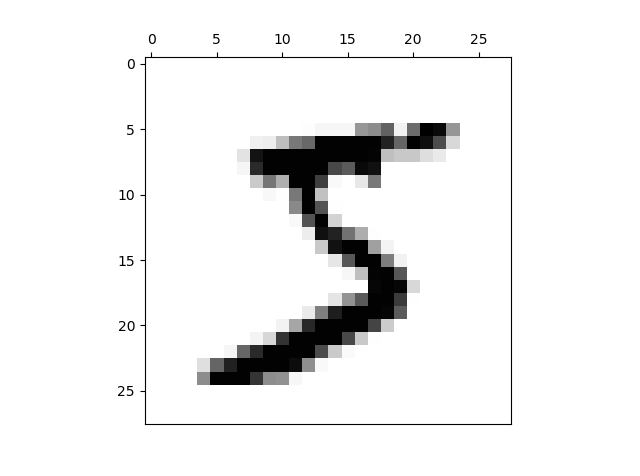
\includegraphics[scale=0.4]{assets/training-0}
  \end{subfigure}%
  ~ 
  \begin{subfigure}[b]{0.4\textwidth}
    \centering
    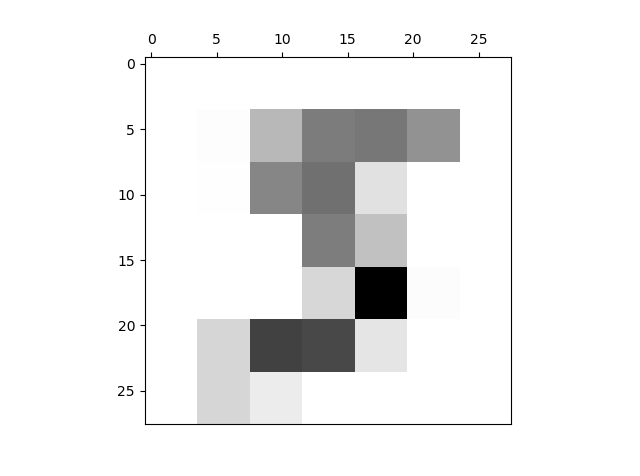
\includegraphics[scale=0.4]{assets/zoning-training-0}
  \end{subfigure}
  \caption{Densité de pixels sur le chiffre 5.}
  \label{fig:zoning}
\end{figure}

On peut généraliser ce procédé en effectuant autre chose qu'une 
moyenne (en général un maximum) et en autorisant les fenêtres 
d'application à se chevaucher. 
C'est ce qui est fait dans les réseaux convolutifs qui seront 
abordés plus loin.
En attendant, on peut observer en figure \ref{fig:zoning-max} 
l'effet de l'utilisation de la fonction \tcode{max} à la 
place de \tcode{mean}. 
Comme on peut le voir, il est plus difficile de reconnaître 
le chiffre.
C'est pourquoi nous utiliserons simplement la densité dans 
nos essais.

\begin{figure}
  \centering
  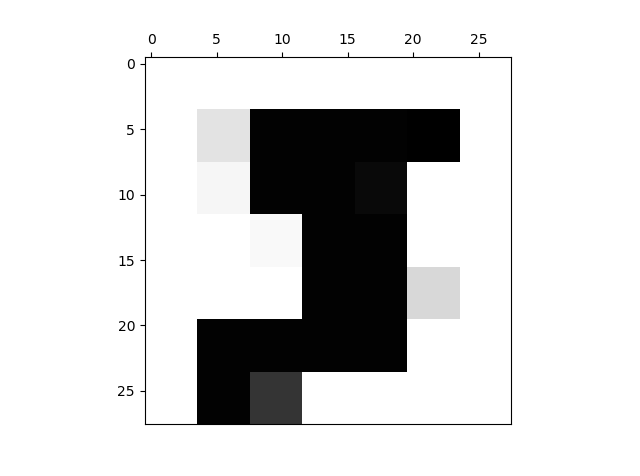
\includegraphics[scale=0.4]{assets/zoning-training-0-max}
  \caption{Filtre \tcode{max} sur des fenêtres non recouvrantes de taille 4x4.}
  \label{fig:zoning-max}
\end{figure}




\section{Nombre de croissements (\nfw{crossings})}



On prend deux points à l’extrémité de l’image et on compte le nombre d’alternance 
entre les groupes de pixels vides et les groupes de pixels contenant de l’encre. 
Cette méthode n’est à priori pas sensible à l’épaisseur du trait.



\section{Histogramme des projections}



On compte pour chaque ligne (resp. chaque colonne) le nombre de pixels allumés sur 
la ligne (resp. colonne). 
En faisant ça sur l’ensemble de l’image, on obtient deux histogrammes. 
Cette technique peut aussi être utilisée pour segmenter des lignes et caractères isolés. 
Cette technique peut être sensible à l’épaisseur du trait. 
Pour palier ce problème, on peut renormaliser chaque histogramme en divisant 
chaque valeur par le total.

\begin{figure}[h]
  \centering
  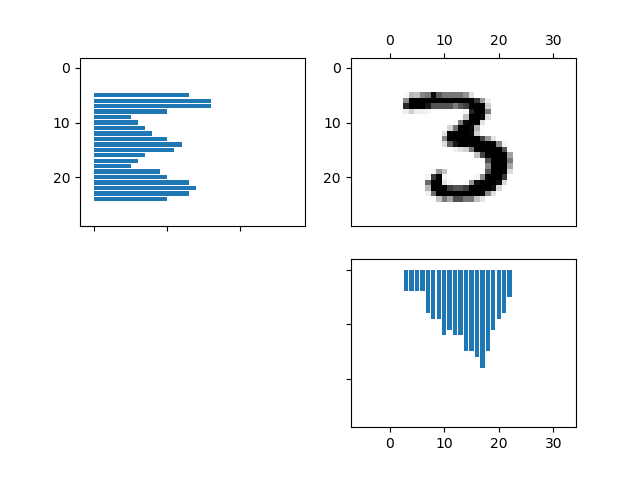
\includegraphics[scale=0.5]{assets/features-hvhisto-ex1}
  \caption{Histogramme des projections du chiffre 3.}
  \label{fig:features-hvhisto-ex1}
\end{figure}



\section{Moments}



Dans tout ce qui suit, on note $p_{xy}$ la valeur du pixel $(x,y)$.

On définit le moment d'ordre $(p+q)$ par:
\[
m_{pq} = \sum_x \sum_y x^p y^q p_{xy}
\]

En pratique, on préférera utiliser des moments centrés (car invariant 
par translation de l'image).
\[
\mu_{pq} = \sum_x \sum_y (x - \overline{x})^p (y - \overline{y})^q p_{xy}
\]
avec 
\[
\overline{x} = \frac{m_{10}}{m_{00}} \qquad \qquad \overline{y} = \frac{m_{01}}{m_{00}}
\]



\section{Transformée de Fourier du contour}

On s'intéresse ici au contour des chiffres comme il est proposé dans \cite{EllipticFourierFeatures}. 
On peut voir le contour comme une fonction périodique 
de $\mathbb{R}$ dans $\mathbb{R}^2$. 
On peut donc lui appliquer une transformée de Fourier pour 
en récupérer un spectre de fréquence. 
En conservant les plus faibles fréquences, on s'intéressera à 
la forme générale du contour sans considérer les détails.

En pratique, on travaille avec un contour discret. 
Dans notre cas, ce contour est stocké en utilisant le codage 
de chaînes de Freeman.
Il s'agit simplement d'un codage indiquant les directions à suivre 
pour tracer le contour (e.g.\/ nord, sub, nord-est, etc...).
Si l'on ajoute à cela un point de départ, on est en mesure de 
reconstruire le contour à partir de la chaîne.


Nous avons implémenté une fonction permettant de calculer le 
contour d'une image.
Voici en quelques mots son principe de fonctionnement. 
On commence par partir du pixel situé en haut à droite de l'image 
et on parcourt les pixels de gauche à droite et de haut en bas 
jusqu'à trouver un pixel colorié. 
On prend comme point de départ le dernier pixel non colorié sur lequel 
on est passé.
On simule ensuite le comportement d'une coccinelle qui serait posée sur 
sur ce pixel et qui serait orientée direction nord-ouest. 
Le but de la coccinelle est d'avancer en maintenant toujours à sa 
droite les pixels coloriés. 
Pour avancer, elle regarde, à partir de sa direction actuelle, quelle 
est la case la plus à droite qu'elle peut atteindre sans faire demi-tour.
Si la première case à droite qu'elle peut atteindre correspond à un demi-tour, 
elle regarde la première case à sa gauche qu'elle peut atteindre
[Note: il y a quelques autres subtilités non décrites ici pour simplifier, 
le code est disponible dans le fichier \tcode{features.py}].
L'algorithme se termine quand la coccinelle revient à son point de départ.

\begin{figure}[h!]
    \centering
    \begin{subfigure}[b]{0.4\textwidth}
        \centering
        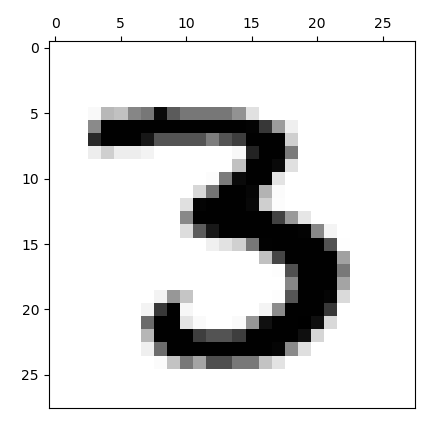
\includegraphics[scale=0.45]{assets/training-image-12}
    \end{subfigure}%
    ~ 
    \begin{subfigure}[b]{0.4\textwidth}
        \centering
        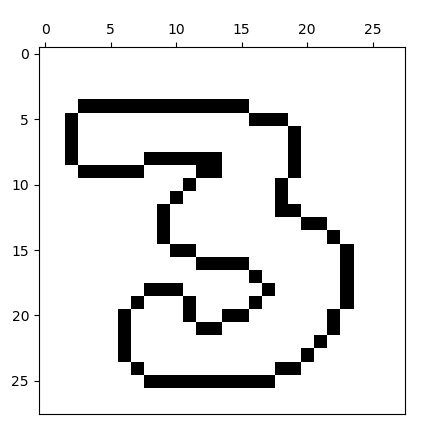
\includegraphics[scale=0.45]{assets/training-image-12-contour}
    \end{subfigure}
    \caption{Contour calculé du chiffre 3.}
\end{figure}

On peut ensuite appliquer une transformée de Fourier à ce contour discret 
et utiliser les coefficients de la décomposition en série de Fourier comme features. 

La figure \ref{fig:contour-reconstruction} montre la reconstruction 
du contour de l'exemple précédent en ajoutant à chaque étape des 
composantes (on commence à l'ordre 1 pour finir à l'ordre 12). 

\begin{figure}[h!]
  \centering
  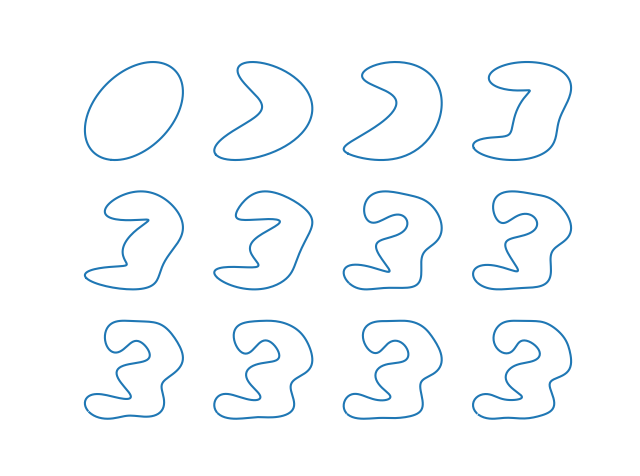
\includegraphics[scale=0.8]{assets/fourier-contour-image12-reconstruction}
  \caption{Reconstruction d'un contour.}
  \label{fig:contour-reconstruction}
\end{figure}

Cette figure permet d'estimer un intervalle d'ordres que l'on pourrait 
utiliser comme feature.



\section{Transformée de Fourier de l'image}

On utilise la fonction \tcode{rfft} de la bibliothèque \tcode{scipy.fftpack} sur 
l'image en niveaux de gris pour passer dans le domaine de Fourier.
La procédure, qui consiste en une double appel à \tcode{rfft}, renvoie une image 
de même taille que l'entrée.

L'image dans le domaine de Fourier est la décomposition de l'image dans le domaine 
fréquentiel.
Il est possible de reconstruire l'image en utilisant la 
fonction \tcode{irfft} de la même bibliothèque.
Cette fonction permet également de visualiser la base utilisée dans le domaine 
fréquentiel (c.f.\/ figure \ref{fig:freq-basis}).

\begin{figure}[h]
  \centering
  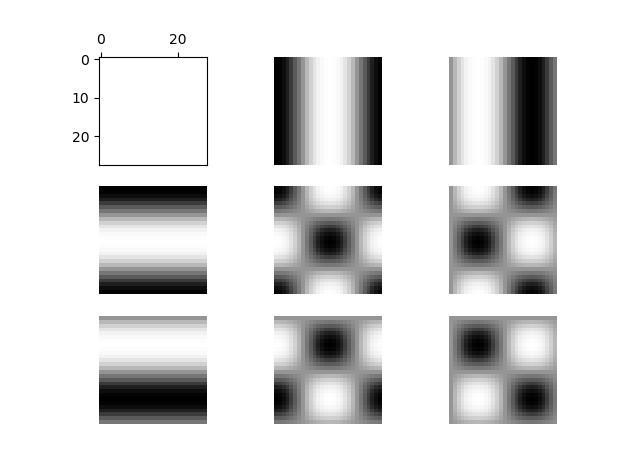
\includegraphics[scale=0.6]{assets/fft-basis}
  \caption{Premiers éléments de la base de Fourier.}
  \label{fig:freq-basis}
\end{figure}

La figure \ref{fig:fft-image-reconstruction} montre la reconstruction d'une 
image en ajoutant progressivement des fréquences.
La figure se lit de gauche à droite et de haut en bas. 
L'image numéro $i$ est reconstruite à partir de tous les coefficients 
d'ordre $p,q < i$ soit $i^2$ coefficients.

\begin{figure}[h]
  \centering
  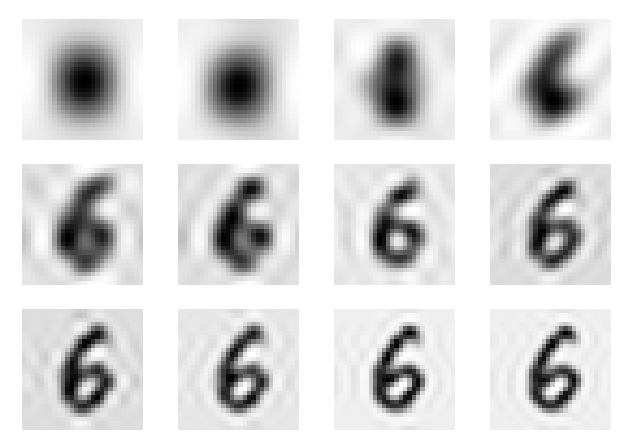
\includegraphics[scale=0.6]{assets/fft-image-num62-reconstruction}
  \caption{Reconstruction d'un $6$.}
  \label{fig:fft-image-reconstruction}
\end{figure}




\section{Reconnaissance avec des techniques de machine learning classiques}

On peut utiliser les features proposées précédemment soit de manière isolée 
soit en groupe pour effectuer de la reconnaissance sur le jeu de test.
Comme le jeu de données est de grande taille (60'000 images), le temps de 
calcul des features est assez important. 
Nous avons donc mis en place un système de cache qui fait que les features ne 
sont calculées qu'une seule fois.

Une fois le calcul des features effectué, on procède de la manière suivante:
\begin{enumerate}
  \item On sélectionne un sous-ensemble des features avec lequel on va entraîner le classifieur;
  \item On entraîne le classifieur avec les données d'entraînement;
  \item On évalue le classifieur sur le jeu de test.
\end{enumerate}

Les features utilisés seront les suivantes:
\begin{itemize}
  \item \tcode{loops}, le nombre de boucles dans l'image;
  \item \tcode{moments}, les moments d'ordre $p+q \leq 4$ (9 valeurs);
  \item \tcode{zones}, les moyennes des patchs de taille $4 \times 4$ (49 valeurs);
  \item \tcode{fourier_contour}, les coefficients de la décomposition en série de Fourier du contour d'ordre $\leq 8$ (32 valeurs);
  \item \tcode{fourier_image}, les coefficients de l'image issue de le transformation \tcode{rfft} présentée précédemment de coordonnées $\leq 4$ (25 valeurs).
\end{itemize}


Dans le cadre de ce projet, nous avons testé différents classifieurs proposés 
par la bibliothèque \tcode{scikit-learn}:
\begin{itemize}
  \item \tcode{KNeighborsClassifier}, un classifieur utilisant l'algorithme des $k$ plus proches voisant;
  \item \tcode{SGDClassifier}, méthode de la descente de gradient stochastique;
  \item \tcode{GradientBoostingClassifier}, méthode du \emph{gradient boosting};
  \item \tcode{RandomForestClassifier}, une forêt aléatoire.
\end{itemize}

La plupart de ces classifieurs sont décrits de manière simple dans la documentation de la bibliothèque.
Pour des explications plus avancées et orientées mathématiques, on pourra par exemple s'orienter 
vers \textit{The Elements of Statistical Learning} \cite{hastie01statisticallearning}.

Chacun de ces classifieurs doit être paramétré (bien qu'il y ait des valeurs par défaut pour les 
paramètres) ce qui rend le travail un peu plus compliqué.
De plus, il convient de bien choisir ses features car, pour certains algorithmes, mélanger 
des features de natures différentes peut avoir des effets néfastes.

Par exemple, l'algorithme des $k$ plus proches voisins de la bibliothèque est optimisé 
dans le cas d'une norme euclidienne (ou plus généralement d'une norme de Minkowski). 
Ainsi, si l'on donne en entrée à l'algorithme des features ayant des ordres de grandeur 
différent, ce sont les variables ayant la plus grande variance que l'algorithme aura 
tendance à privilégier (et pas forcément les plus pertinentes).
Ce problème peut être atténué en normalisant les données d'entrées (ce qui n'est pas 
toujours pertinent).

Nous commençons d'abord par tester les différents classifieurs avec les 
paramètres par défaut pour voir lesquels sont les plus prometteurs.
Cela correspond par exemple à 10 estimateurs pour les forêts aléatoires
et à 5 voisins pour les $k$ plus proches voisins.
Le tableau suivant montre les résultats obtenus (pourcentage d'images bien classées dans le 
jeu de test) en fonction des features utilisés et d'une éventuelle renormalisation ($\sigma = 1$).
Certains algorithmes étant en partie aléatoires, les résultats peuvent varier 
légèrement d'un essai à l'autre.

\begin{table}[h]
\centering
\begin{tabular}{cccccc}
 \hline
 Features                & $\sigma=1$    & KNN    & SGD   & GB    & RF \\
 \hline
 \tcode{loops}           &  \tcode{True} &  20,66 & 14,86 & 23,13 & 23,13 \\
 \tcode{moments}         &  \tcode{True} &  74.77 & 56.5  & 75.27 & 75.79 \\
 \tcode{zones}           &  \tcode{True} &  94.39 & 87.71  & 93.62 & 93.45 \\
 \tcode{fourier_contour} &  \tcode{True} &  93.61 & 53.18 & 92.05 & 93.72 \\
 \tcode{fourier_image}   &  \tcode{True} &  93.66 & 85.67 & 91.66 & 90.12  \\
\end{tabular}
\caption{Classification à l'aide d'une seule feature.}
\label{table:machine-learning-1}
\end{table}

Comme on peut le voir, on peut déjà arriver à des résultats satisfaisants en choisissant
bien une feature et un classifieur.

On peut alors avoir envie de tester plusieurs stratégies pour améliorer les résultats:
\begin{enumerate}
  \item garder la feature qui semble la plus prometteuse, et améliorer le paramétrage des classifieurs;
  \item ne pas toucher au paramétrage des classifieurs, mais considérer plusieurs features;
  \item faire une combinaison des deux points précédents.
\end{enumerate}


\begin{table}[h]
\centering
\begin{tabular}{ccccccc}
 \hline
 Feature A               & Feature B               & $\sigma=1$    & KNN    & SGD   & GB    & RF \\
 \hline  
 \tcode{loops}           & \tcode{moments}         &  \tcode{True} & 78.98 & ? & ? & 79.74 \\
 \tcode{loops}           & \tcode{moments}         & \tcode{False} & 69.41 & ? & ? & 79.91 \\
 \tcode{loops}           & \tcode{zones}           &  \tcode{True} & 95.28 & ? & ? & 93.76 \\
 \tcode{loops}           & \tcode{zones}           & \tcode{False} & 95.42 & ? & ? & 94.09 \\
 \tcode{zones}           & \tcode{fourier_image}   &  \tcode{True} & 94.92 & ? & ? & 93.4 \\
 \tcode{zones}           & \tcode{fourier_image}   & \tcode{False} & 95.43 & ? & ? & 93.61 \\
\end{tabular}
\caption{Classification avec deux features.}
\label{table:machine-learning-2}
\end{table}

L'agrégation des deux features permet d'obtenir des résultats légèrement meilleurs. 
Cela est d'autant plus marqué lorsque les features ne permettent pas séparément d'obtenir 
de bons résultats.
La deuxième ligne du tableau permet de voir l'effet que peut avoir la non-renormalisation des 
entrées sur le $k$ plus proches voisins.
Ce dernier n'est cependant pas systématique comme on peut le voir deux lignes en dessous.
Sans surprise, le RandomForest est beaucoup moins affecté par l'absence de renormalisation.


\begin{table}[h]
\centering
\begin{tabular}{ccccccc}
 \hline
 Feature A               & Feature B               & $\sigma=1$    & 10    & 25    & 50    & 100 \\
 \hline  
 \tcode{zones}           & \tcode{fourier_image}   & \tcode{False} & 93.47 & 94.82 & 95.24 & 95.33 \\
\end{tabular}
\caption{Effet de la variation du nombre d'estimateurs de la RandomForest.}
\label{table:machine-learning-rf-n-estimators}
\end{table}

\chapter{Reconnaissance basée sur les réseaux convolutionnels}






\chapter{Comparaison des résultats}




TODO : on pourra dans cette partie comparer les résultats avec des méthodes qui ne sont pas 
basés sur des réseaux de neurones.

\begin{appendices}


\end{appendices}


\backmatter

\printindex


\newpage

\renewcommand{\leftmark}{Bibliographie}
\bibliography{bib} 
\bibliographystyle{abbrv}




\end{document}
